\documentclass[10pt]{article}
\usepackage[letterpaper,text={6.5in,8.7in},centering]{geometry}
\usepackage{amssymb,amsmath,times,url,subfigure,graphicx,multirow}
\usepackage[pdftex,urlcolor=blue,pdfpagemode=none,pdfstartview=FitH]{hyperref}
\usepackage[final]{pdfpages}
\usepackage{biblatex}
\addbibresource{library.bib}
%% url smaller font.
\makeatletter
\def\url@leostyle{%
  \@ifundefined{selectfont}{\def\UrlFont{\sf}}{\def\UrlFont{\small\ttfamily}}}
\makeatother
\urlstyle{leo}

%\usepackage[all,import]{xy}


\renewcommand{\baselinestretch}{1.2}
\date{}

\renewcommand{\thesubsection}{\arabic{subsection}. }
\renewcommand{\thesubsubsection}{\arabic{subsection}.\arabic{subsubsection} }


\begin{document}
\pagestyle{empty}
\section*{MAE 3145: Orbital Mechanics \& Space Dynamics}
\vspace*{-0.4cm}
\noindent{Fall 2016, MW 12:45-2:00pm, SEH 3040}

%From 2012, Delete Chapter 5, and revise the course calendar.

\paragraph*{Instructor}
Shankar Kulumani\quad Email: \href{mailto:skulumani@gwu.edu}{skulumani@gwu.edu}\quad Homepage: \url{http://fdcl.seas.gwu.edu/}\\
\hspace*{1.8cm}
Office Hour: TBD or by appointments at SEH 2200


\paragraph*{Prerequisites} APSC 2058 Analytical Mechanics II

\paragraph*{Course Description} This course covers the motion of spacecraft under gravity. Included are the derivation and the analyses of the two-body problem and their applications for real world missions.
Extensive use of scientific programming languages is required to simulate orbital dynamics and solve real-world astrodynamics problems.

\paragraph*{Textbook}
\begin{list}{$\bullet$}{\setlength{\itemsep}{-3pt}}\item 
H. Curtis, \textit{Orbital Mechanics: for Engineering Students}, 2nd Edition, Elsevier 2010\\
(Ebook is available through the Gelman Library.)
\item R. Bate, \textit{Fundamentals of Astrodynamics}, Dover Publication, 1971
\end{list}


\paragraph*{Contents}
\begin{list}{$\bullet$}{\setlength{\itemsep}{-3pt}}
\item Astrodynamic Fundamentals
    \begin{list}{$-$}{\setlength{\itemsep}{-3pt}}
    \item Time [Curtis Chap. 5.4, BMW Chap. 2.9]
    \item Coordinate Systems [Curtis Chap. 4, BMW Chap. 7.4]
    \item COMFIX
    \end{list}
\item Orbital Mechanics\vspace*{-0.2cm}
    \begin{list}{$-$}{\setlength{\itemsep}{-3pt}}
    \item Dynamics of Point Masses [Curtis Chap. 1]
    \item Two-Body Problem [Curtis Chap. 2,3, BMW Chap. 1]
    \item Orbital Elements [Curtis Chap. 4, BMW Chap. 2.3]
    \item Groundtracks [Curtis Chap. 4.8, BMW Chap. 2.15]
    \item RV2COE
    \item PROPOGATE
    \end{list}
%\item Orbit Determination\vspace*{-0.2cm}
%    \begin{list}{$-$}{\setlength{\itemsep}{-3pt}}
%    \item Gibbs Method [Chap. 5]
%    \end{list}
\item Orbital Maneuvers\vspace*{-0.2cm}
    \begin{list}{$-$}{\setlength{\itemsep}{-3pt}}
    \item Hohmann Transfers [Curtis Chap. 6, BMW Chap. 3]
    \item Plane Changes [Curtis Chap. 6.9, BMW Chap. 3.4]
    \item Orbital Rendezvous and Phasing [Curtis Chap. 6.5, BMW Chap. 8.3]
    \end{list}
\item Perturbations
    \begin{list}{$-$}{\setlength{\itemsep}{-3pt}}
    \item Geopotential [Curtis Chap. 4.7]
    \item Drag
    \item PREDICT
    \end{list}
\end{list}

\paragraph*{Software Projects}
A major focus of this course will be the application of sound scientific programming skills.
You will apply the theoretical tools of astrodynamics to solve realistic problems by implementing your own library of tools.

\begin{list}{$\bullet$}{\setlength{\itemsep}{-3pt}}
    \item COMFIX - determine the orbital elements of a satellite given ground based radar observations
    \item RV2COE - convert position and velocity vectors of a spacecraft to classical orbital elements
    \item PROPOGATE - determine the position of a satellite as a function of time
    \item PREDICT - predict satellite passes for any location on the Earth
    \end{list}
\paragraph*{Additional Readings}
\begin{list}
{$\bullet$}
{\setlength{\itemsep}{-3pt}}
\item \fullcite{vallado2007}
\item \fullcite{battin1999}
\item J. Danby, \textit{Fundamentals of Celestial Mechanics}, Willmann-Bell, 1988
\item J. Prussing, \textit{Orbital Mechanics}, Oxford University Press, 1993
\item V. Chobotov, \textit{Orbital Mechanics}, AIAA, 2002
\item T. Logsdon, \textit{Orbital Mechanics: Theory and Applications}, Wiley, 1997
%%\item R. Dorf, and R. Bishop, \textit{Modern Control Systems}, Prentice Hall, 2007
%\item K. Ogata, \textit{Modern Control Engineering}, Prentice Hall, 2001
%\item N. Leonard and W. Levine, \textit{Using MATLAB to Analyze and Design Control Systems}, Addison Wesley, 1995
\item MATLAB Tutorial by Mathworks: \url{http://www.mathworks.com/academia/student_center/tutorials/}
\item Scipy Tutorial: \href{http://www.scipy-lectures.org/}{http://www.scipy-lectures.org/}
%\item MATLAB Control System Toolbox Getting Started Guide by Mathworks:\\ \url{http://www.mathworks.com/access/helpdesk/help/pdf_doc/control/get_start.pdf}
\end{list}
%\renewcommand{\thesubfigure}{}
%\begin{figure}[h]\vspace*{-0.3cm}
%\centerline{
%\subfigure[Etkin]{
%    \href{http://books.google.com/books?id=AIIOAAAACAAJ}%
%    {\includegraphics[height=2.3cm]{etkin.pdf}}}
%\subfigure[Nelson]{
%    \href{http://books.google.com/books?id=bt46AAAACAAJ}%
%    {\includegraphics[height=2.3cm]{nelson.jpg}}}
%\hspace*{0.5cm}
%\subfigure[Stevens]{
%    \href{http://books.google.com/books?id=T0Ux6av4btIC}%
%    {\includegraphics[height=2.3cm]{stevens.jpg}}}
%\subfigure[Stengel]{
%    \href{http://books.google.com/books?id=nI_EHQAACAAJ&dq=stengel+flight&ei=YpKkSL7tL4L2iQG7hZ36BA}%
%    {\includegraphics[height=2.3cm]{stengel.jpg}}}
%\subfigure[Roskam]{
%    \href{https://oscommerce.darcorp.com/product_info.php?cPath=21&products_id=125&osCsid=077f051b037aa4a35b9b6e52998bbae8}%
%    {\includegraphics[height=2.3cm]{roskam.jpg}}}
%\hspace*{0.5cm}
%\subfigure[Anderson]{
%    \href{http://books.google.com/books?id=Hd_AR0CAmsoC}%
%    {\includegraphics[height=2.3cm]{anderson.jpg}}}
%\subfigure[McClamroch]{
%    \href{http://my.fit.edu/~taeyoung/McClamroch.pdf}%
%    {\includegraphics[height=2.3cm]{nhm.pdf}}}}
%\end{figure}

\paragraph*{Grading}
Homework 35\%,\;\; Attendance 5\%,\;\; Midterm Exam 20\% ,\;\; Final Exam 20\%, \;\; Projects 20\%


\paragraph*{Course Learning Objectives}
At the end of this course, students will be able to:

\newcounter{lcounter}
\begin{list}
{\arabic{lcounter}:}
{\setlength{\itemsep}{-3pt}\usecounter{lcounter}}
\item Explain the Newtonian gravitational force and gravitational potential between particles
%\item Understand the dynamics of a system of two particles acting under their mutual gravitational potential
\item Analyze the characteristics of circular, elliptic, parabolic and hyperbolic orbits in a two-dimensional plane
\item Describe the geometry of an orbit in a three-dimensional space from orbital elements
\item Apply numerical/analytical techniques to propogate orbits.
\item Choose and apply the approprite orbital maneuvering method to move spacecraft between orbits.
\item Develop personal software tools to solve practical astrodynamic problems:
    \begin{itemize}
        \item Determine orbital parameters from ground based observations.
        \item Predict satellite passes and determine observation angles to view satellites overhead.
    \end{itemize}
\end{list}



\paragraph*{Course Calendar\footnote{This calendar is subject to revision. In particular, the section references are only a guide, and your instructor may deviate from it.}}
$ $

\vspace*{0.3cm}

\centerline{\small\selectfont
\begin{tabular}{|c|c||p{2.9cm}|p{2.1cm}|p{2.9cm}|p{2.1cm}|p{2.1cm}|}\hline
Month & Week & \textbf{M} & {Tu} & \textbf{W} & Th & F \\ \hline\hline
\multirow{2}{0.8cm}{\centering{August}} 
 & \multirow{2}{0.8cm}{\centering{1}} 
 & 28 & 29 & 30 & 31 & 1 \\ 
\raisebox{0cm}[0.5cm][0.1cm]{}&& 
\S 1.3-1.4 - \textbf{HW0}&  & \S1.5  & & \\\hline
%
\multirow{7}{0.8cm}{\centering{Sept}} 
 & \multirow{2}{0.8cm}{\centering{2}} 
 & 4 & 5 & 6& 7& 8 \\ 
\raisebox{0cm}[0.5cm][0.1cm]{}&& 
Labor day & & Matlab  & & \\\cline{2-7}
%
 & \multirow{2}{0.8cm}{\centering{3}} 
 & 11 & 12 & 13 & 14 & 15 \\ 
\raisebox{0cm}[0.5cm][0.1cm]{}&& 
Matlab & & \S 2.3 & & \\\cline{2-7}
%
 & \multirow{2}{0.8cm}{\centering{4}} 
 & 18 & 19 & 20 & 21 & 22  \\ 
\raisebox{0cm}[0.5cm][0.1cm]{}&& 
\S2.4 & & \S 2.6 & & \\\cline{2-7}
%
 & \multirow{2}{0.8cm}{\centering{5}} 
 & 25 & 26 & 27 & 28 & 29 \\ 
\raisebox{0cm}[0.5cm][0.1cm]{}&& 
\S2.7-2.9 \textbf{COMFIX} & & \S 2.9-3.2 & & \\\hline
%% Oct
\multirow{8}{0.8cm}{\centering{Oct}} 
 & \multirow{2}{0.8cm}{\centering{6}} 
 & 2 & 3 & 4& 5 & 6   \\ 
\raisebox{0cm}[0.5cm][0.1cm]{}&& 
\S3.3-3.6 & & \S 4.2-4.3 & & \\\cline{2-7}
%
 & \multirow{2}{0.8cm}{\centering{7}} 
  & 9 & 10 & 11 & 12 & 13 \\ 
\raisebox{0cm}[0.5cm][0.1cm]{}&& 
Fall Break \S4.4 & Fall Break & \S 4.7 & & \\\cline{2-7}
%
 & \multirow{2}{0.8cm}{\centering{8}} 
  & 16 & 17 & 18 & 19 & 20\\ 
\raisebox{0cm}[0.5cm][0.1cm]{}&& 
\S 6.2-6.3 & & \textbf{Midterm} & & \\\cline{2-7}
%
 & \multirow{2}{0.8cm}{\centering{9}} 
  & 23 & 24 & 25 & 26 & 27 \\ 
\raisebox{0cm}[0.5cm][0.1cm]{}&& 
\textbf{RV2COE} &  & \S 6.4  & & \\\hline
%% Nov
\multirow{8}{0.8cm}{\centering{Nov}} 
 & \multirow{2}{0.8cm}{\centering{10}} 
 & 30 & 31 & 1 & 2 & 3 \\ 
\raisebox{0cm}[0.5cm][0.1cm]{}&& 
\S 6.5-6.6 & & \S6.7 & & \\\cline{2-7}
%
 & \multirow{2}{0.8cm}{\centering{11}} 
  & 6 & 7 & 8 & 9 & 10 \\ 
\raisebox{0cm}[0.5cm][0.1cm]{}&& 
\S 6.8  & & \S6.10  & & \\\cline{2-7}
%
 & \multirow{2}{0.8cm}{\centering{12}} 
  & 13 & 14 & 15 & 16 & 17\\ 
\raisebox{0cm}[0.5cm][0.1cm]{}&& 
\S 8.2 & & \S8.3 & & \\\cline{2-7}
%
 & \multirow{2}{0.8cm}{\centering{13}} 
  & 20 & 21 & 22 & 23 & 24  \\ 
\raisebox{0cm}[0.5cm][0.1cm]{}&& 
\textbf{PROPOGATE} &  & Thanksgiving & Thanksgiving & Thanksgiving\\\hline
%
 & \multirow{2}{0.8cm}{\centering{14}} 
 & 27 & 28 & 29 & 30 & 1  \\ 
\raisebox{0cm}[0.5cm][0.1cm]{}&& 
\S8.6-8.8 & & \S 2.12 &  & \\\cline{2-7}
%%
\multirow{3}{0.8cm}{\centering{Dec}} 
 & \multirow{2}{0.8cm}{\centering{15}} 
 & 4 & 5 & 6 & 7 & 8   \\ 
\raisebox{0cm}[0.5cm][0.1cm]{}&& 
\S 2.12 &  & \S 2.12  & & \\\cline{2-7}
%
 & \multirow{2}{0.8cm}{\centering{16}} 
 & 11 & 12 & 13 & 14 & 15 \\ 
\raisebox{0cm}[0.5cm][0.1cm]{}&& 
\textbf{PREDICT} & Reading Day & Finals begin &  & \\\hline%\cline{2-7}
%
% & \multirow{2}{0.8cm}{\centering{17}} 
% & 14 & 15 & 16 & 17 & 18 \\ 
%\raisebox{0cm}[0.5cm][0.1cm]{}&& 
% &  &  & Final exams end & \\\hline
\end{tabular}}

\newpage
\paragraph*{General Policy}
\begin{list}
{\arabic{lcounter}:}
{\setlength{\itemsep}{-3pt}\usecounter{lcounter}}

\item \textbf{Check your GW email account daily}. All of the important announcements of this class will be made through your email. 



\item All examinations, papers, and other graded work products and assignments are to be completed in conformance with The George Washington University Code of Academic Integrity (available at \url{http://www.gwu.edu/~ntegrity/code.html}).

\item If you do not have a computer account for accessing Python, you should contact SEAS Computing Facility

\item You may need to take notes during class apart from the handouts handed out. Make sure to carry a notebook or a laptop for this purpose.

\item Class attendance is required. Be punctual and follow the class rules. Students are encouraged to ask questions but talking while the lecture is being delivered is prohibited.

\item Homework assignments should be prepared in a neat and professional manner. Discussion of assignments and collaboration among students is  encouraged; however,  each student is expected to prepare each assignment problem solution by himself/herself. Do not copy. Use of solutions manuals is prohibited.

\item Late homework assignment will not be accepted.
    Your lowest homework grade will be dropped and not count towards the final grade.

\item No excuse on missing exams will be accepted. Make-up exams will not be given, except under extraordinary circumstances such as documented illness. If an exam is simply missed, then a grade of zero will be recorded. If you shall have a conflict of schedule, you must inform the instructor in writing with supporting documents at least a week ahead of time.

\item If you shall have any questions regarding grading, you must attach to your paper a written explanation and give them to instructor within one week after the paper is returned.

\item If you shall have any questions regarding the course, you should see Dr. Nigam during his office hours or contact him via email.
\item Set cell phone to silent mode in the classroom and refrain from texting.
 
\item Class/Lab cancellation due to weather or special event: Call 202-994-5050 or visit the Campus Advisories Website (\url{campusadvisories.gwu.edu}) or \url{www.gwu.edu/~bygeorge/100703/closingpolicy.html} for GW operating status. 

\item Disability Support Services (DSS): If a student is to use DSS for testing, he/she should submit the letter from DSS during the first week. Any student who may need an accommodation based on the potential impact of a disability should contact the Disability Support Services office (\url{http://gwired.gwu.edu/dss/}) during the first week.

\item Students requiring special accommodations for testing through DSS must provide Dr. Lee with the appropriate forms or documents and confirm the approval at least two weeks before the test or exam.
\end{list}
\paragraph*{To Report an Emergency or Suspicious Activity}

Call the GW Police Department at 202-994-6111 (Foggy Bottom). If the line is unavailable or you are calling from another University location or off campus, dial 911.


\paragraph*{Shelter in Place - General Guidance}

Your first reaction in an emergency should be to stay where you are. Evacuate only if you hear the fire alarm or someone instructs you to evacuate. If you are outdoors during an incident, proceed into the closest GW building unless you are told to do otherwise. No matter where you are on campus, the basic steps of sheltering in place are:

\begin{list}
{\arabic{lcounter}:}
{\setlength{\itemsep}{-3pt}\usecounter{lcounter}}

\item	Shelter-in-place in an interior room, above ground level, and with the fewest windows. If there is a large group of people inside a particular building, several rooms may be necessary.
\item	Shut and lock all windows (locking will form a tighter seal), close exterior doors, and stay away from glass doors and windows.
\item	Turn off air conditioners, heaters, and fans. Close vents to ventilation systems as you are able (Facilities staff will turn off ventilation systems as quickly as possible).
\item	Make a list of the people with you and call the list in to GWPD (see numbers above) so they know where you are.
\item	Visit GW Campus Advisories \url{http://CampusAdvisories.gwu.edu} or call the GW Information Line at 202-994-5050 for incident updates. If possible, turn on a radio or television and listen for further instructions. If your e?mail address or mobile device is registered with Alert DC, check for alert notifications.
\item	Make yourself comfortable and look after one other. You will get word as soon as it is safe to come out.
\end{list}

\paragraph*{Evacuation}

We will always evacuate if the fire alarm sounds or if the building we are in becomes unsafe. In the event of an evacuation, please quickly gather your personal belongings (purse, keys, cell phone, GWorld card, etc.) and proceed to the nearest exit. Do not use the elevator.

Once we have evacuated the building, proceed to the east entrance of SEH. If the first location is not available, we will meet at Marvin Center (800 21st Street, in the lobby)


\paragraph*{Alert DC \& GW Alert}
Alert DC provides free notification by e-mail or text message during an emergency. Visit GW Campus Advisories for a link and instructions on how to sign up for alerts pertaining to GW. If you receive an Alert DC notification during class, please share the information immediately.
 

GW Alert provides popup notification to desktop and laptop computers during an emergency. In the event that we receive an alert to the computer in our classroom, we will follow the instructions given. You are also encouraged to download this application to your personal computer. Visit GW Campus Advisories to learn how. Additional  information  about  emergency  preparedness  at  GW  can  be  found  on  GW  Campus  Advisories \url{http://CampusAdvisories.gwu.edu}.
 

\paragraph*{University Policy on Religious Holidays}
\begin{list}
{\arabic{lcounter}:}
{\setlength{\itemsep}{-3pt}\usecounter{lcounter}}

\item Students should notify faculty during the first week of the semester of their intention to be absent from class on their day(s) of religious observance. 
\item Faculty should extend to these students the courtesy of absence without penalty on such occasions, including permission to make up examinations. 
\item Faculty who intend to observe a religious holiday should arrange at the beginning of the semester to reschedule missed classes or to make other provisions for their course-related activities
\end{list}

\paragraph*{Support for Students Outside the Classroom}

\begin{itemize}
\item Disability Support Services (DSS)

Any student who may need an accommodation based on the potential impact of a disability should contact the Disability Support Services office at 202-994-8250 in the Rome Hall, Suite 102, to establish eligibility and to coordinate reasonable accommodations. For additional information please refer to: \url{http://disabilitysupport.gwu.edu}

\item Mental Health Services 202-994-5300	

The University's Mental Health Services offers 24/7 assistance and referral to address students' personal, social, career, and study skills problems. Services for students include: crisis and emergency mental health consultations confidential assessment, counseling services (individual and small group), and referrals.  \url{http://counselingcenter.gwu.edu}

\end{itemize}



%\paragraph*{Academic Integrity Code}
%
%Academic dishonesty is defined as cheating of any kind, including misrepresenting one's own work, taking credit for the work of others without crediting them and without appropriate authorization, and the fabrication of information. For the remainder of the code, see: \url{http://studentconduct.gwu.edu/code-academic-integrity}
%
%
%\paragraph*{Email Policy}
%
%\begin{list}
%{$\bullet$}
%{\setlength{\itemsep}{-3pt}}
%\item \textbf{Check your GW email account daily}. All of the important announcements of this class will be made through your email. 
%
%\item I will not respond to emails which are composed in an unprofessional manner, or which violates basic email etiquette. Think professional business letter to a potential employer, as opposed to a text message to your friend.
%
%\item Before sending an email inquiry, please carefully review the syllabus and course website to ensure that your question has not been addressed there. Questions that have been addressed in the syllabus or on the course website will receive responses that redirect you back to the appropriate resource.
%
%\item I do not offer immediate round the clock technical support, please plan ahead accordingly.
%I will try to respond to emails within 36 hours during the week, and within 72 hours during the weekend.
%\end{list}
%
%\paragraph*{Homework Policy}
%
%\begin{list}
%{$\bullet$}
%{\setlength{\itemsep}{-3pt}}
%
%\item Homework will be due at the \textbf{beginning of class}. \textbf{Late homework will not be accepted}. If you plan on being absent on a day that a homework set is due, you may either turn it in earlier or have a friend turn it in for you.
%
%\item Grading of the homework will emphasize your effort to present the solution in a near and orderly fashion.
%\begin{list}
%{$-$}
%{\setlength{\itemsep}{-3pt}}
%\item Use one side of a clean paper (graphed or lined is okay) that is not torn from a spiral notebook.
%\item Write your name, ID number, and section clearly on the front page of your completed assignment.
%\item Clearly number each solution and present them in numerical order.
%\item Leave at least one line of space between each problem.
%\item Write clearly and legibly.
%\item Use a stapler.
%\end{list}
%
%\item Please keep all your exams and homeworks; if you believe there has been an error in the recording of your grades they are the only way to validate your claim.
%
%\item A student may discuss homework problems with other students to develop and clarify his/her approach. But, the written solution should be an independent and individual effort that reflects his/her own understanding of the problem. As a general guide, a student should be able to independently reproduce any submitted solution. \textbf{Copying or allowing another student to copy your work or solution manual is considered cheating}.
%\end{list}
%
%\paragraph*{Exam Policy}
%
%\begin{list}
%{$\bullet$}
%{\setlength{\itemsep}{-3pt}}
%
%%\item \textbf{No make-up quizzes will be given.} However, your lowest quiz score will be dropped.
%
%\item There are one midterm exam and final exam. \textbf{Make-up exams will not be given except in exceptional circumstances} such as family emergency or medical emergency. In emergency situations, students should notify the occurrences \textbf{as early as possible}, and students will be expected to provide \textbf{a certified document} such as a doctor's letter indicating the nature and time of the medical emergency.
%
%\end{list}
%
%
%
%

\paragraph*{Academic Expectations for University Courses\footnote{Zucker, Steven, \textit{Teaching at the University Level}, AMS Notices (43), 1996, pp 863-865. Available at
\url{http://www.ams.org/notices/199608/comm-zucker.pdf}}}

\begin{list}
{$\bullet$}
{\setlength{\itemsep}{-3pt}}

\item You are no longer in high school. The great majority of you, not having done so already, will have to discard high school notions of teaching and learning and replace them by university-level notions.  Our goal is more than just getting you to reproduce what was told to you in the classroom.

\item Expect to have material covered at two to three times the pace of high school. Above that, we aim for greater command of the material, especially the ability to apply what you have learned to new situations (when relevant).

\item Lecture time is at a premium, so it must be used efficiently. You cannot be \textit{taught} everything in the classroom. It is your responsibility to learn the material. Most of this learning must take place outside the classroom. You should be willing to put in two hours outside the classroom for each hour of class.

\item The instructor's job is primarily to provide a framework, with some of the particulars, to guide you in doing your learning of the concepts and methods that comprise the material of the course. It is not to \textit{program} you with isolated facts and problem types nor to monitor your progress.

\item You are expected to read the textbook for comprehension. It gives the detailed account of the material of the course. It also contains many examples of problems worked out, and these should be used to supplement those you see in the lecture. 

%However, there is the clear advantage that you can read it at your own pace. Use pencil and paper to work through the material and to fill in omitted steps.
%As for when you engage the textbook, you have the following dichotomy:
%[recommended for most students] Read for the first time the appropriate section(s) of the book before the material is presented in lecture. That is, come prepared for class. Then the faster-paced college-style lecture will make more sense.
%If you haven't looked at the book beforehand, try to pick up what you can from the lecture (absorb the general idea and/or take thorough notes) and count on sorting it out later while studying from the book outside of class.

\item Exams will consist largely of \textit{fresh} problems that fall within the material that is being tested.

\end{list}

\newpage



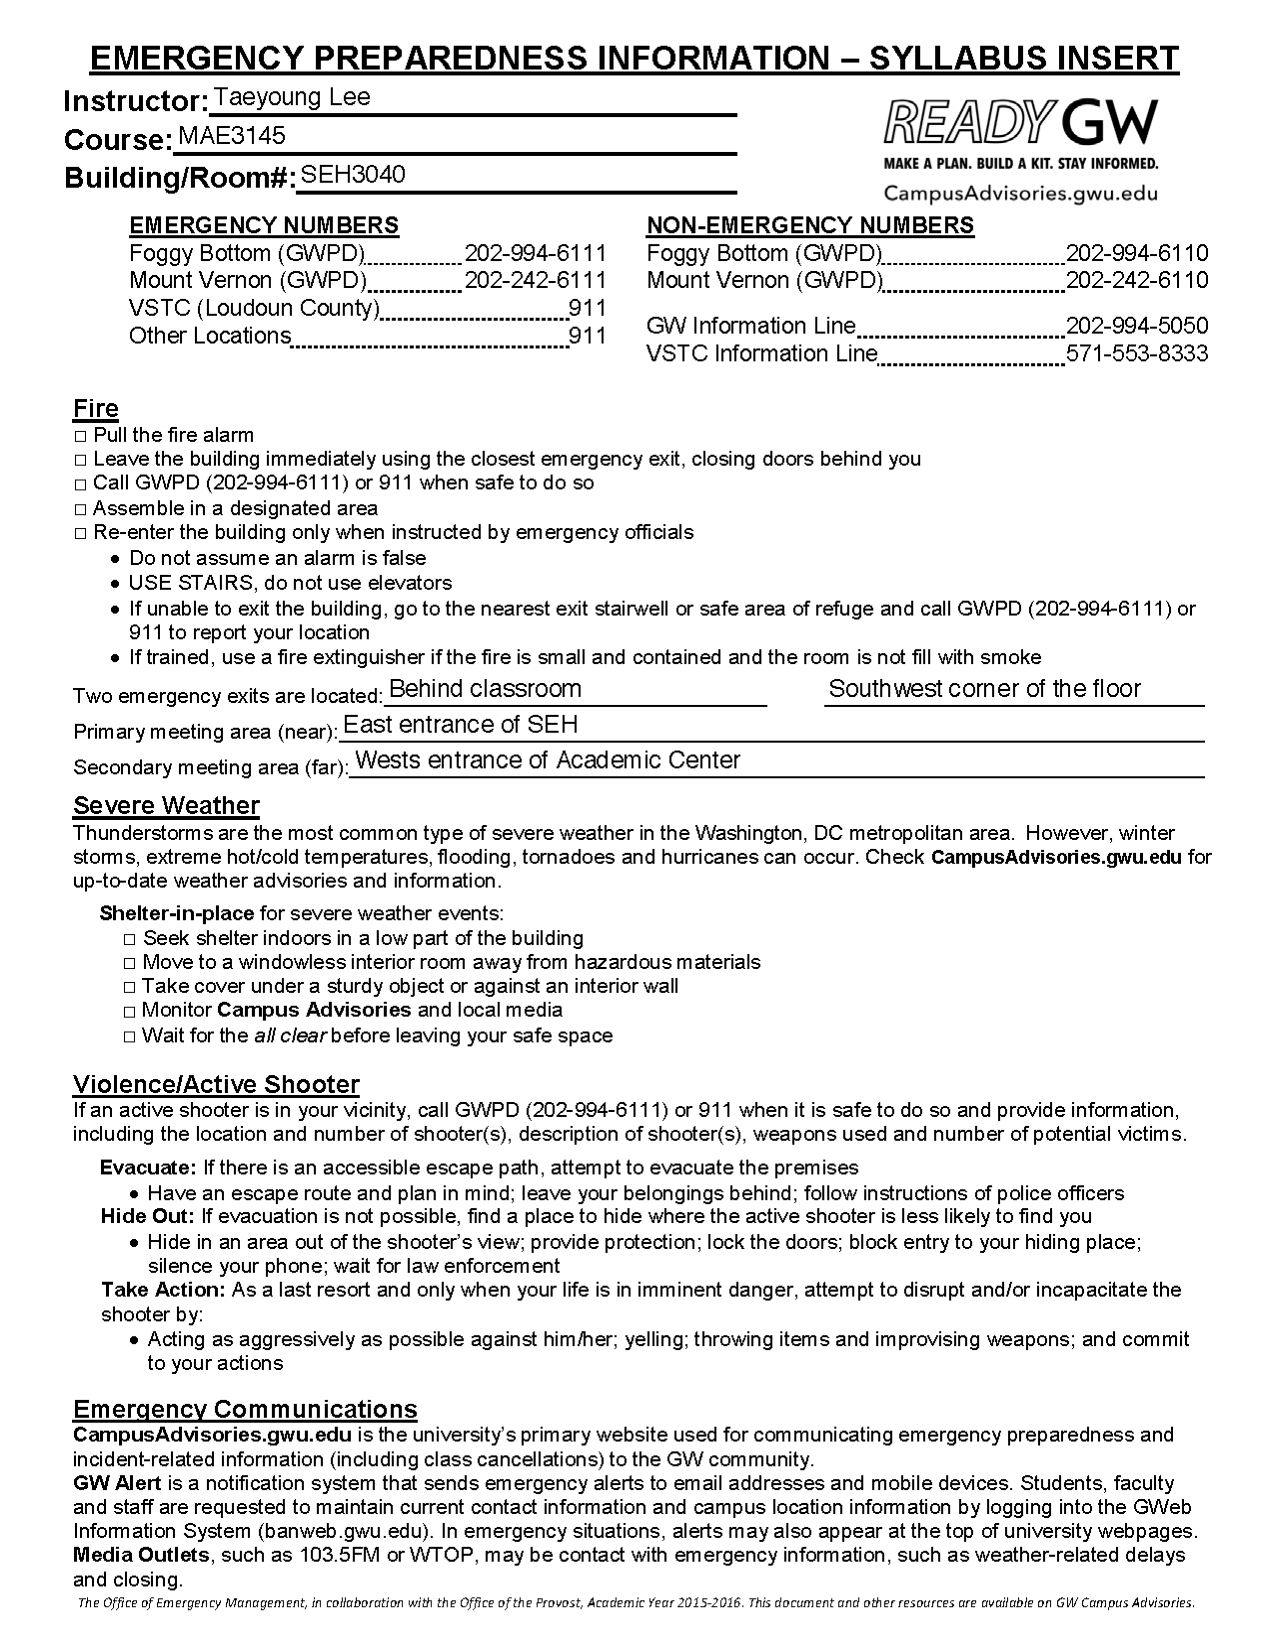
\includepdf{Syllabus_Insert_MAE3145_0}
\end{document}

